\newcommand{\graphwidth}{6.2cm}


\section{Accuracy of modelfitting}

\subsection{Ranges and resolutions}

One of the major problems faced throughout the development of the modelfitting algorithm was with the selection of ranges and resolutions.
In Listing \ref{leastsquarescode} there is a mention of four variables - $range_\theta$, $range_\alpha$, $resolution_\theta$ and $resolution_\alpha$.
These variables control the size and resolution of the parameter space that is searched during the modelfitting.
Care must be taken when adjusting these variables as they control both the accuracy of the results and the execution time of the algorithm.

Some of the problems encountered when selecting values for the variables are discussed below.

\begin{figure}[p]
	\centering
	\subfloat[Left thigh energy]{\label{Alpha:GoodLeftThigh}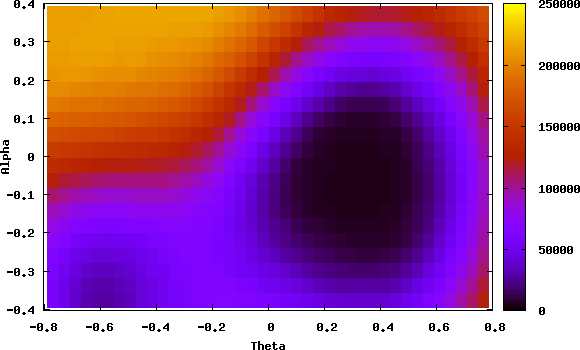
\includegraphics[width=\graphwidth]{problems/good-leftthigh.png}}
	\qquad
	\subfloat[Right thigh energy]{\label{Alpha:GoodRightThigh}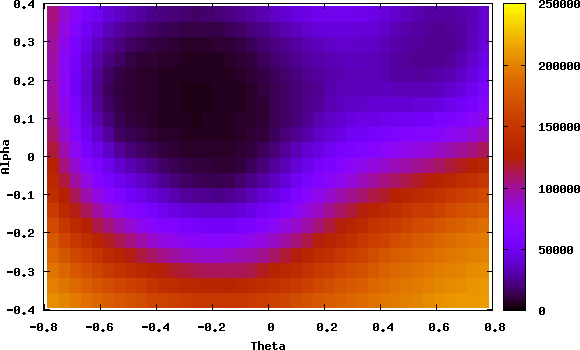
\includegraphics[width=\graphwidth]{problems/good-rightthigh.png}}
	\\
	\subfloat[Left lower leg energy]{\label{Alpha:GoodLeftLower}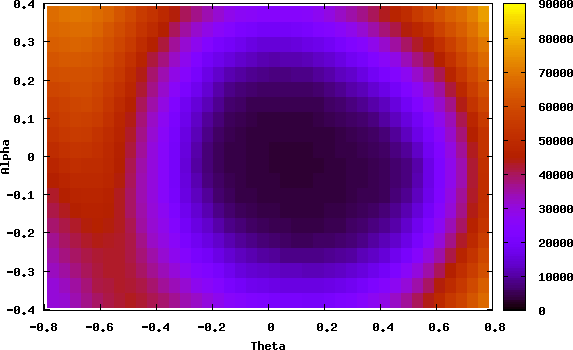
\includegraphics[width=\graphwidth]{problems/good-leftlower.png}}
	\qquad
	\subfloat[Right lower leg energy]{\label{Alpha:GoodRightLower}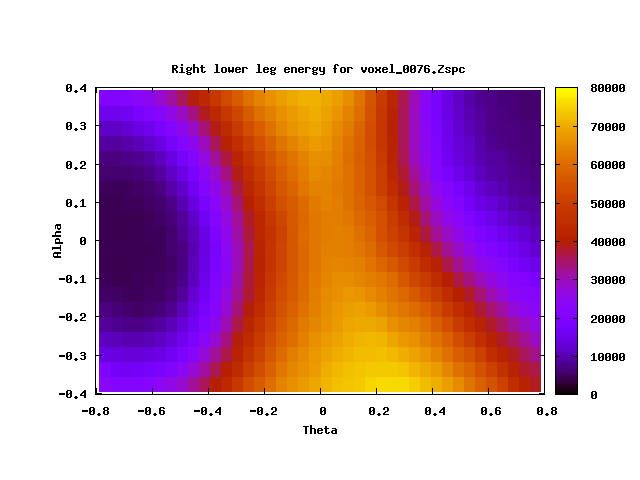
\includegraphics[width=\graphwidth]{problems/good-rightlower.png}}
	\\
	\subfloat[Model and voxel data]{\label{Alpha:Good3D}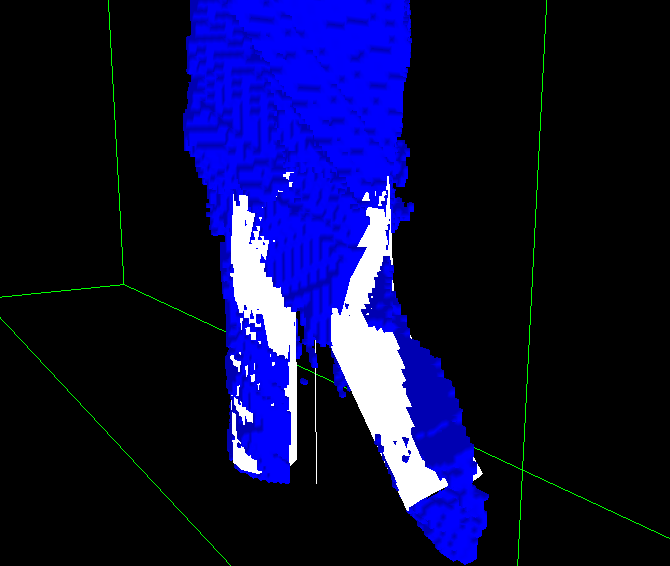
\includegraphics[width=\graphwidth]{problems/good-3d.png}}
	\qquad
	\subfloat[Model]{\label{Alpha:GoodModel}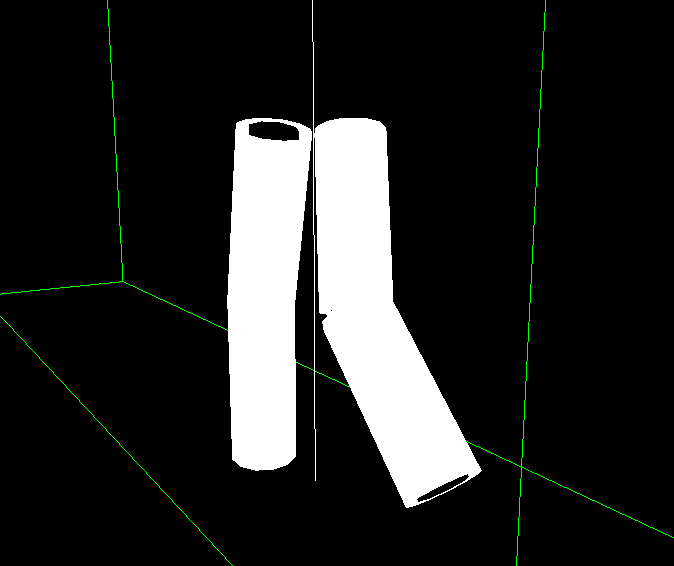
\includegraphics[width=\graphwidth]{problems/good-model.png}}
	
	\caption{Frame 76, a good fitting of the model to the data.
		Notice in \ref{Alpha:GoodRightThigh} how there is a local minimum developing in the upper-right corner.
		Remember that \ref{Alpha:GoodRightThigh} and \ref{Alpha:GoodRightLower} are slices through a four-dimensional space,
		and as such there may be minima elsewhere that are not shown.}
	\label{AlphaGood}
\end{figure}

\begin{figure}[p]
	\centering
	\subfloat[Left thigh energy]{\label{Alpha:BadLeftThigh}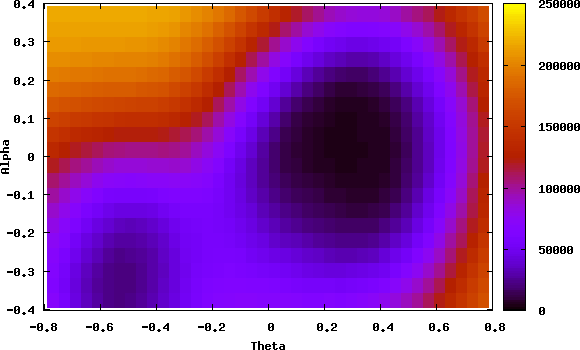
\includegraphics[width=\graphwidth]{problems/badalpha-leftthigh.png}}
	\qquad
	\subfloat[Right thigh energy]{\label{Alpha:BadRightThigh}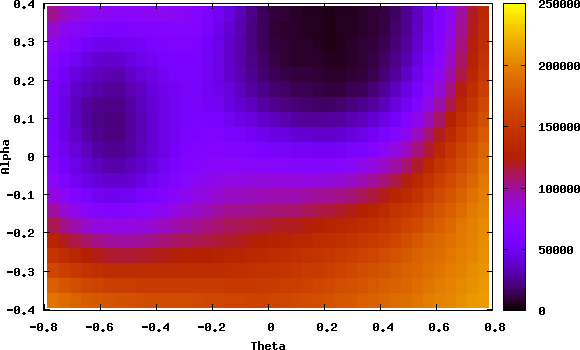
\includegraphics[width=\graphwidth]{problems/badalpha-rightthigh.png}}
	\\
	\subfloat[Left lower leg energy]{\label{Alpha:BadLeftLower}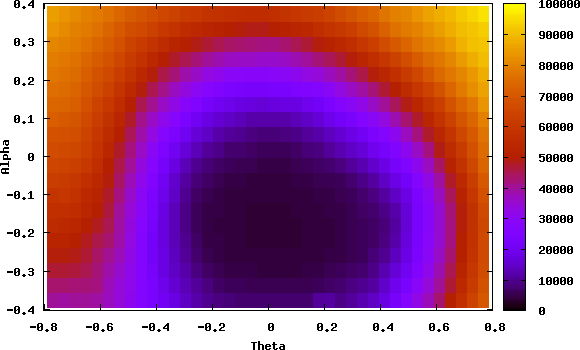
\includegraphics[width=\graphwidth]{problems/badalpha-leftlower.png}}
	\qquad
	\subfloat[Right lower leg energy]{\label{Alpha:BadRightLower}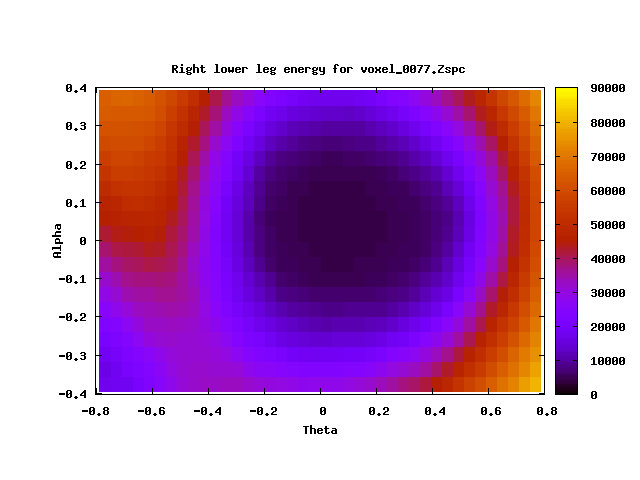
\includegraphics[width=\graphwidth]{problems/badalpha-rightlower.png}}
	\\
	\subfloat[Model and voxel data]{\label{Alpha:Bad3D}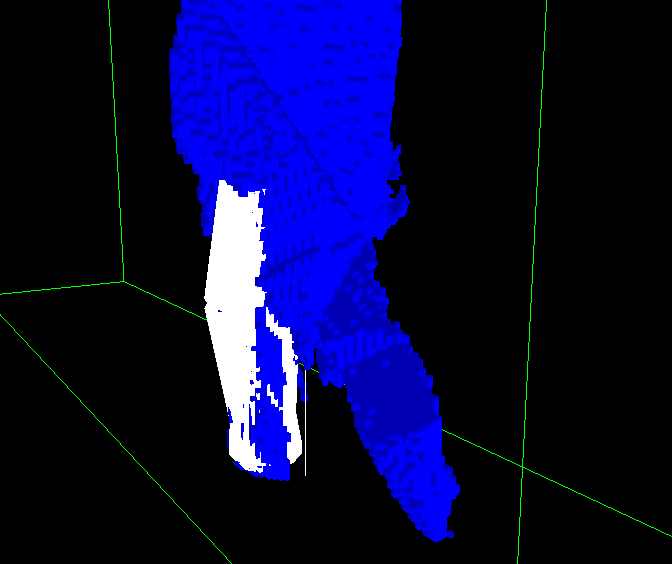
\includegraphics[width=\graphwidth]{problems/badalpha-3d.png}}
	\qquad
	\subfloat[Model]{\label{Alpha:BadModel}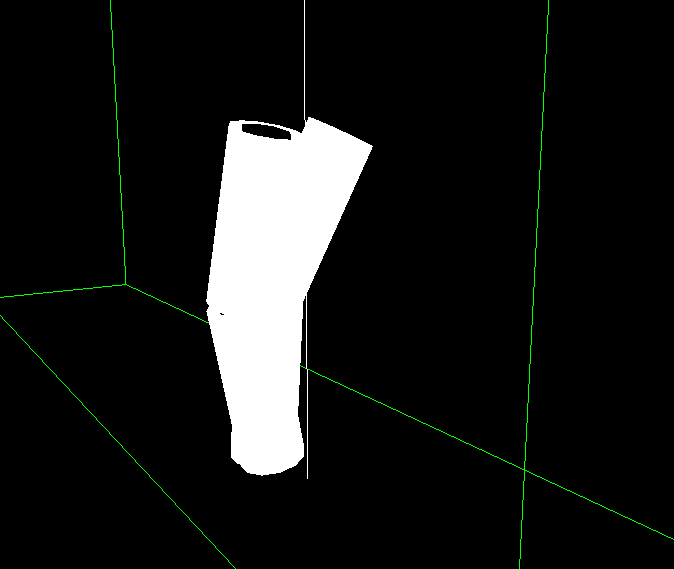
\includegraphics[width=\graphwidth]{problems/badalpha-model.png}}
	
	\caption{Frame 77, an erroneous fitting of the model to the data.
		The local minimum in \ref{Alpha:GoodRightThigh} on the previous page must have had a much lower energy with $(\alpha_2, \theta_2) = (0, 0)$ (lower leg energy).
		In this frame the energy at that point became even lower - lower than that of the correct point - and became the global minimum.}
	\label{AlphaBad}
\end{figure}

\begin{enumerate}
	\item \textbf{Erroneous minima}.
		Originally we had set $range_\alpha = \left[ -\frac{\pi}{8}, +\frac{\pi}{8}\right]$.
		This range turned out to be far too big, and as such would lead to erroneous minima being found.
		The problem tended to occur when the two thighs were close together - one of the thighs would assume
		a large alpha value and swing towards the subject's other leg.
		The two leg models would then intersect as they matched the same leg in the data.
		
		Figures \ref{AlphaGood} and \ref{AlphaBad} demonstrate this problem.
		They are of subsequent frames in sample 81 - the first frame matches the right leg correctly
		but the second frame is incorrect.
		The right thigh has an alpha value that is strongly positive, and this leads to it matching most of the left leg instead.
		
		To understand why this has happened we need to remember that the parameter space is four-dimensional, and each of the energy plots
		shown are only slices with two of the parameters held constant.
		Therefore much of the parameter space is not shown in the plots.
		Figure \ref{Alpha:GoodRightThigh} shows a small low energy region near the top, in a similar location to the larger low energy region in Figure \ref{Alpha:BadRightThigh}.
		The energy of this region in the first plot is not nearly as low as the other, correct, minimum, so we may wonder why it has grown so dramatically between frames.
		The answer is that Figure \ref{Alpha:GoodRightThigh} is a slice at the minimum in Figure \ref{Alpha:GoodRightLower} - if we moved it so the slice
		were instead taken at the minimum from Figure \ref{Alpha:BadRightLower} we would likely see a much stronger low energy region.
		
		This was a major problem, and a number of approaches were taken to attempt to solve it.
		The first was to smooth the data - using the results of the previous frames to apply a penalty to parameters that were too far away from the expected position.
		However this seemed more like a remedy to the result of the problem (wrong minima being chosen) rather than the cause of it (bad alpha range).
		Also it was feared that any kind of smoothing of the data might destroy valuable gait information.
		
		Instead it was decided to take the simpler solution - limiting the range of possible alpha values.
		A strong divide was noted between the typical alpha values of correct and incorrect frames - the correct frames all took on
		values within the range $\left[ -\frac{\pi}{32}, +\frac{\pi}{32}\right]$, and the others outside.
		$range_\alpha$ was therefore set to $\left[ -\frac{\pi}{32}, +\frac{\pi}{32}\right]$.
	
	\item \textbf{Oversampling}.
		There is a limit to the maximum resolution at which it is sensible to sample the parameter space.
		The size of the voxels in the data is $1\text{cm}^3$.
		Comparing the fitting of two orientations of the model that differ by less than $1\text{cm}^3$ is meaningless,
		as the coordinates of every distance lookup performed are clamped to integer values (not doing so would break
		the lookup cache from Section \ref{Optimisations:LookupCache}).
		
		Sampling at these high resolutions could not be considered before multi-resolution sampling was implemented
		as the execution time would have been prohibitive.
		With the introduction of multi-resolution sampling however some high-resolution fittings were tested, and as expected
		the noise resulting from the discrete nature of the data led to errors in the DFT and a lower classification rate.
		
		The ideal resolutions were discovered to be $resolution_\theta = 21$ and $resolution_\alpha = 11$ - meaning the
		parameter space is 21x21x11x11 (odd numbers were chosen to ensure there is one sample taken at $(0, 0, 0, 0)$).
\end{enumerate}


\subsection{Quantitative error analysis}
\label{Modelfitting:ErrorAnalysis}

A manual fitting was produced for selected samples to provide a means of evaluating the error of the modelfitting algorithm.
Each frame was examined in the modelfitting application, and the parameters of the model tweaked to visually fit the model to the image of the subject.
Samples 81 and 96 were chosen for this manual fitting process as they gave very different success rates in classification.
Sample 81 is one of the samples of Subject 1, who was classified correctly in most of the tests.
Sample 96 is one of the samples of Subject 4, who was never classified correctly in any of the tests.

Figures \ref{ManualFit81:res10}, \ref{ManualFit96:res10}, \ref{ManualFit81:res20}, \ref{ManualFit96:res20}, \ref{ManualFit81:multires}, \ref{ManualFit96:multires} show the differences between parameter values for automatic fitting and manual fitting,
and Table \ref{ManualFitTable} summarises this information in tabular form.
Only the $\theta$ values were compared as their errors affect classification far more than those in the $\alpha$ values.

The error between the manually entered result $m_t$ and the automatically determined result $a_t$ for a sample with $N$ frames was calculated as follows:

\begin{equation}
	E = \frac{1}{N} \sum_{t=1}^N \left| a_t - m_t \right|
\end{equation}

The values in the table below represent the average error per frame as a percentage of the possible range for $\theta$ ($\pm \frac{\pi}{4}$).

\begin{table}[thb]
	\centering
	\begin{tabular}{l|cc|cc|cc}
		& \multicolumn{2}{|c|}{Low fixed res} & \multicolumn{2}{|c|}{High fixed res} & \multicolumn{2}{|c}{Multi-resolution} \\
		& 81 & 96 & 81 & 96 & 81 & 96 \\
		\hline
		Left thigh & 2.94\% & 1.83\% & 3.18\% & 1.97\% & 3.01\% & 1.48\% \\
		Right thigh & 2.23\% & 2.45\% & 2.33\% & 2.39\% & 2.70\% & 1.98\% \\
		Left lower leg & 6.37\% & 5.17\% & 6.02\% & 4.68\% & 5.34\% & 2.78\% \\
		Right lower leg & 3.81\% & 5.21\% & 3.56\% & 4.86\% & 4.15\% & 3.98\% \\
		\hline
		Overall & 3.84\% & 3.66\% & 3.77\% & 3.48\% & 3.80\% & 2.56\% \\
		Mean error & \multicolumn{2}{|c|}{3.75\%} & \multicolumn{2}{|c|}{3.62\%} & \multicolumn{2}{|c}{3.18\%} \\
	\end{tabular}
	\caption{Overview of the average error per frame for different modelfitting algorithms.}
	\label{ManualFitTable}
\end{table}

\begin{figure}[p]
        \centering
        \subfloat[Left thigh]{\label{ManualFit81:res10:LeftThigh}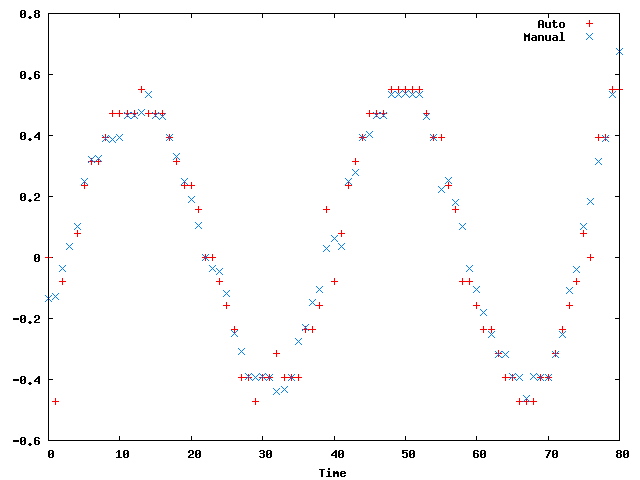
\includegraphics[width=\graphwidth]{manualfitting/81-res10-leftthigh.png}}
        \quad
        \subfloat[Right thigh]{\label{ManualFit81:res10:RightThigh}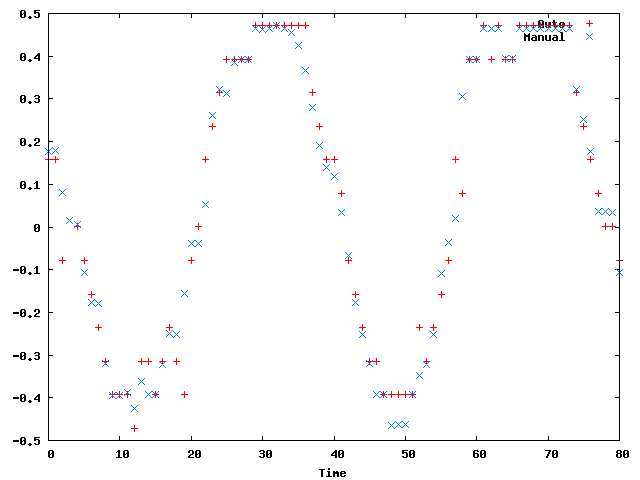
\includegraphics[width=\graphwidth]{manualfitting/81-res10-rightthigh.png}}
        \
        \subfloat[Left lower leg]{\label{ManualFit81:res10:LeftLower}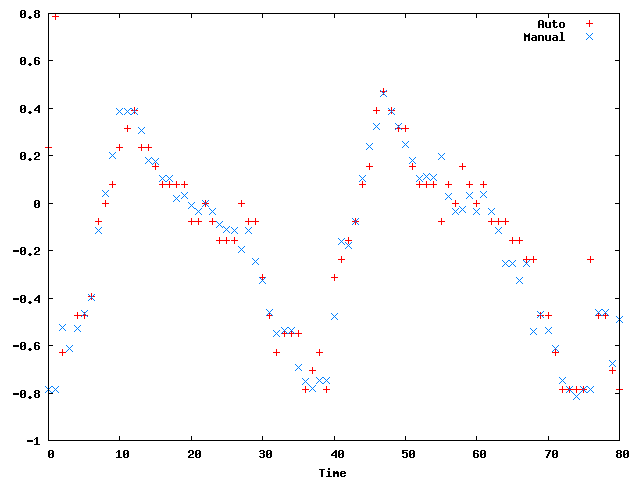
\includegraphics[width=\graphwidth]{manualfitting/81-res10-leftlower.png}}
        \quad
        \subfloat[Right lower leg]{\label{ManualFit81:res10:RightLower}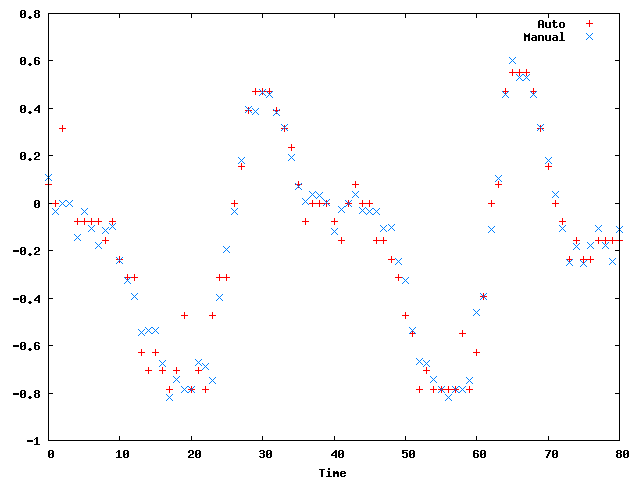
\includegraphics[width=\graphwidth]{manualfitting/81-res10-rightlower.png}}

        \caption{Fitting error for Sample 81 using the low fixed resolution search.}
        \label{ManualFit81:res10}
\end{figure}


The overall low error rate for the modelfitting is encouraging.
As is to be expected, the lower resolution search is not quite as accurate as the high resolution search.
The multi-resolution search seems to perform even better, as its second pass has twice the equivalent resolution of the high fixed resolution search.
The low error rate for multi-resolution is particularly encouraging as it was a concern in section \ref{Design:MultiRes} that the algorithm might ``home in'' on some non-global minima and miss the true fitting.

Comparing the error rates between the samples is suprising, since Sample 81 fared so much better in classification than Sample 96, but seems to have a higher error.
One possible explanation for this relates to the way in which classification operates.
Two of the four samples from each subject are classified manually and the remaining two undergo automatic classification.
A success is recorded if the automatic classification matches either of the two manually labelled samples.
It could be that the modelfitting algorithm fit Sample 96 well, but was less successful with the other three samples from the same subject.

This suggests that classification might depend more on the structure of the feature space than the accuracy of modelfitting.

\bigskip
\noindent So how might we account for the errors in the fitting?
There are several obvious possibilities - the first of which is noise in the 3D voxel data.
The modelfitting algorithm seems to cope fairly well with noisy data - one of the worst samples is shown in Figure \ref{BadData}, but despite the holes in the subject's legs and spurious groups of surrounding voxels the algorithm still manages to correctly fit the model.

Another possibility is that the subject's clothing might interfere with correct fittings to the data.
The modelfitting algorithm tries to place the cylinders in the model in the centre of groups of voxels - where the distance between the edges of the model and the edge voxels are equal on all sides.
Baggy trousers that move around as the subject walks will confuse the algorithm, as it will try to place the cylinders in the centre of the trousers, which may not be the same as the centre of the leg.
A possible solution to this problem is presented in Section \ref{FutureWork:BaggyTrousers}.

\begin{figure}[bp]
	\centering
	\subfloat[Voxel data]{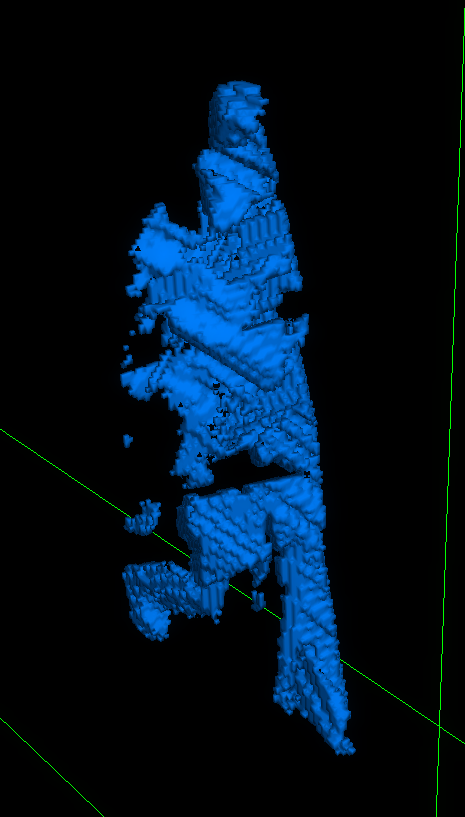
\includegraphics[height=8cm]{baddata/voxels.png}}
	\quad
	\subfloat[Model]{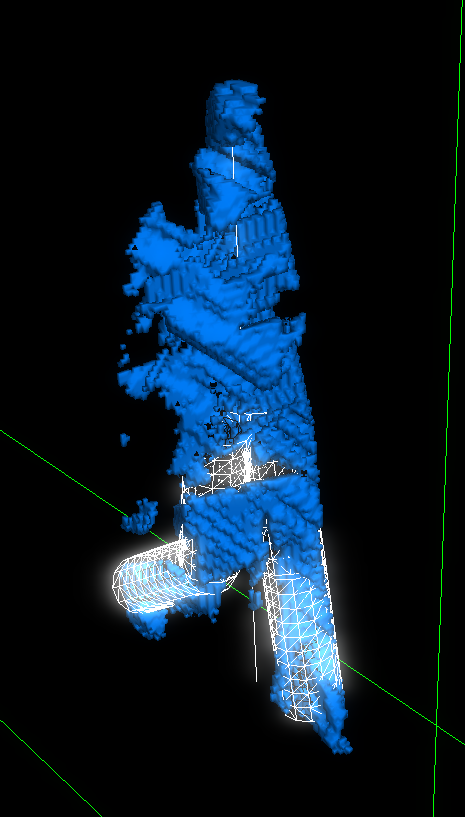
\includegraphics[height=8cm]{baddata/model.png}}
	
	\caption{One of the worst examples of 3D reconstruction.}
	\label{BadData}
\end{figure}

There are certain cases where our model for the human leg seems inadequate for describing the data.
In Figure \ref{FittingErrors} we see that our automatic fitting algorithm has missed the true shape of the subject's right leg, and instead has placed the model in an incorrect location that still matches a large number of voxels.
When trying to manually fit this frame, we see that a correct value for the thigh's $\theta$ leads to the lower leg being too far forward to properly match its voxels.
There are two explanations for this - the first is that the thigh in our model is too long.
While it would explain the results seen in this frame, there are plenty of other frames in which the thigh appears to be of the correct length.
The other explanation is that the lower leg is pivoting about the leg at the wrong point.
If we allowed it to rotate about a point slightly further up the thigh then it may stand a better chance of matching the data.


\begin{figure}[bp]
	\centering
	\subfloat[Automatic fitting]{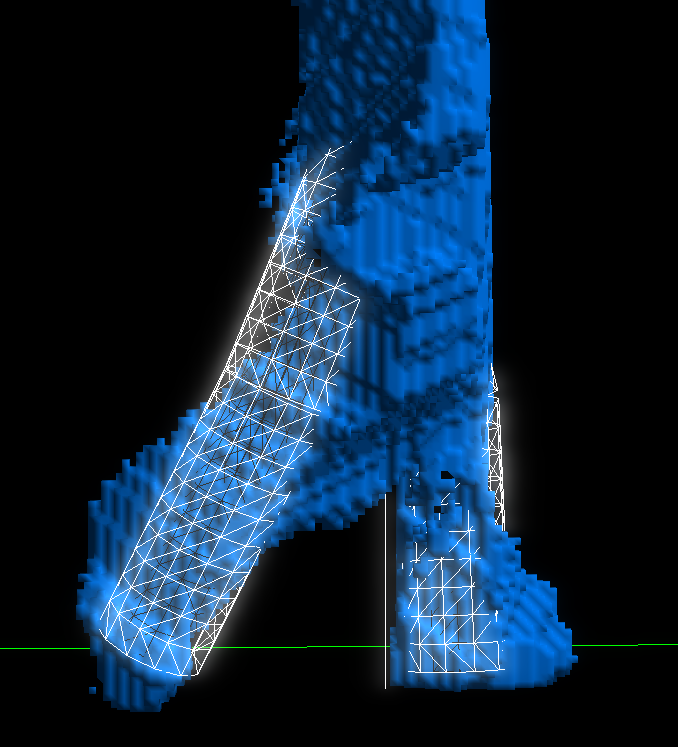
\includegraphics[width=6cm]{fittingerrors/model.png}}
	\quad
	\subfloat[Manual fitting]{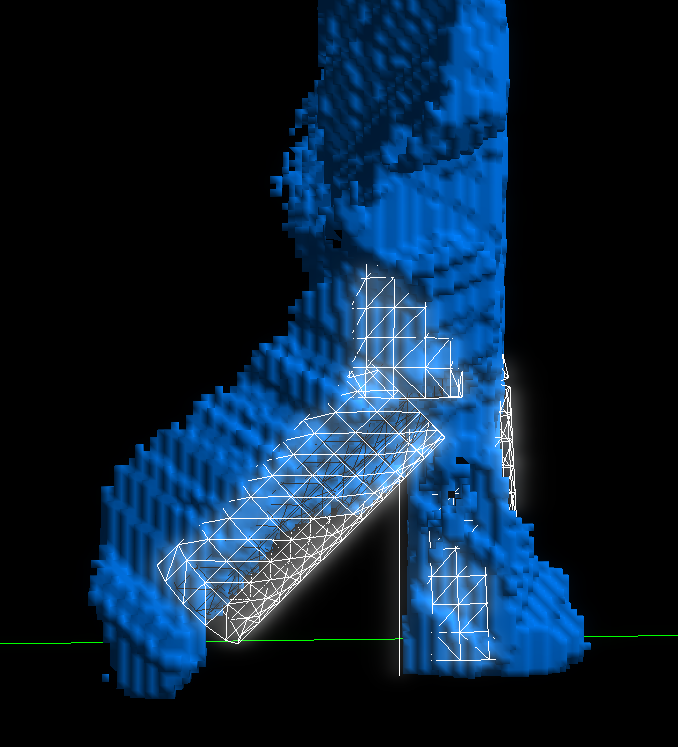
\includegraphics[width=6cm]{fittingerrors/manualmodel.png}}
	
	\caption{Sometimes our model of the human leg does not adequately describe the data.
		In Sample 81 Frame 77 the thigh is too long and the lower leg cannot properly match the subject.}
	\label{FittingErrors}
\end{figure}
